\section{Introduction}
\label{sec:intro}

An agentic LLM session is not a request. It is a long-lived job that issues a
round of inference, waits on a tool, and comes back---tens of times---with a
context that grows every round. On a memory-constrained accelerator this makes
admission control look like the obvious lever. The KV pool is the binding
resource; a single large session can occupy most of it; and the sessions
themselves are wildly heterogeneous. If a scheduler can see how much of the
pool a candidate will need and how much room is left, surely it should beat a
fixed number.

We believed this, built a controller that does exactly that, and spent a
considerable amount of GPU time discovering that on our workload and hardware
it is false. This paper reports the negative result, but its contribution is
not the negative result---it is the decomposition that explains it, and the
boundary that decomposition draws.

\subsection{What we measured}

We serve a replay of 200 real coding-agent sessions on a single RTX 3090
(Qwen2.5-Coder-7B, 96K context, SGLang, a 101{,}432-token KV pool) and compare
a family of admission policies against a sweep of static concurrency caps.
Nine controller variants, spanning four mechanistically distinct ideas, all
land on or below the static Pareto front (Fig.~\ref{fig:frontier}). The best
of them reaches the front and no further.

\begin{figure}[tb]
  \centering
  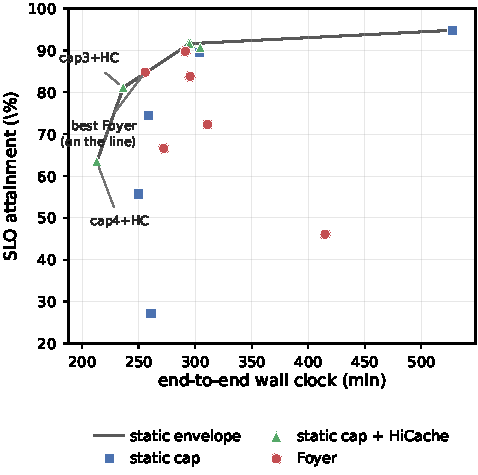
\includegraphics[width=\columnwidth]{figs/fig1_frontier.pdf}
  \caption{Every completed run on the (wall clock, SLO) plane. The grey line
  is the upper-left envelope of the static points; a policy below or on it has
  not beaten a static cap, because time-slicing two caps approximates any
  point on the segment between them. Nine controller variants, none above.}
  \label{fig:frontier}
\end{figure}

\subsection{Why}

We decompose the wall clock into \emph{busy} time, during which the engine has
at least one request in flight, and \emph{idle} time, during which it has
none. The busy component is governed by
\begin{equation}
  W_{\text{busy}} \;\approx\; \frac{\text{output tokens}}{\overline{R}}\; \times\; \tau,
  \label{eq:model}
\end{equation}
where $\overline{R}$ is the mean number of running requests and $\tau$ is the
per-step cost. An admission policy controls $\overline{R}$ and nothing else.
The difficulty is that $\tau$ is not constant in $\overline{R}$: we observe it
rise by 20--25\% in exactly the two configurations that push concurrency
hardest, and the rise cancels the gain from the extra concurrency.

The idle component is structural rather than a control failure. A session in a
tool wait issues no request, so when all live sessions happen to be waiting,
the engine is genuinely empty---and we measure that stretches of 5--25\,s of
zero occupancy are common. Crucially, the tool wait itself is much longer than
the trace's median suggests: the median inter-round gap is 0.35\,s, but the
\emph{mean} is 16.85\,s with 22\% of gaps over ten seconds. A controller that
reads only the median concludes, as we initially did, that sessions never
leave and therefore that there is no idle time to recover. There is.

\subsection{Contributions}

\begin{itemize}
  \item We falsify, with pre-registered criteria, four mechanistically
        distinct routes by which an adaptive admission controller was expected
        to beat a tuned static cap on this workload: changing the accounting
        base, changing the growth reserve, changing the hard ceiling, and
        changing the execution granularity from session-count to
        running-request-count. Each is reported with its measured reason
        (\S\ref{sec:results}).
  \item We give a two-part decomposition of the wall clock (\S\ref{sec:model})
        that explains all of the above with one mechanism: admission policy
        moves the running-request count, and the per-step cost moves with it.
  \item We characterize when adaptivity \emph{could} have paid, and show that
        our workload is not that case: the same throttle configuration that is
        worth $+51\%$ at 25 sessions costs $-42\%$ at 200 (\S\ref{sec:load}).
        Put differently, no single scalar cap is optimal across both, which is
        the regime adaptive control exists for---and we measure that adaptive
        control does not reach it either, because the aggregator's own
        accounting error is load-independent.
  \item We make the measurements reproducible: the verdict of every run is
        produced by a single script from the raw per-step logs, and we report
        the three claims we had to retract along the way, with the checks that
        caught them.
\end{itemize}

\subsection{What we do not claim}

We do not claim that admission control is useless in general. We claim it does
not pay \emph{here}, we show the measurement that decides it, and we argue
(\S\ref{sec:discussion}) that the same measurement can be taken on another
workload in minutes. We also do not claim our hardware and model are
representative; our results are from one 24\,GB accelerator and one 7B model,
and extending them is future work.
